\documentclass[11pt]{article}

%4pp das transps
% psnup -W415 -H273 -s.9 -b10 -d10 -c -4 05-Tecnicas_Compressao_Imagens.ps 05-Tecnicas_Compressao_Imagens.4pp.ps

\usepackage[utf8]{inputenc} % PARA USAR PALAVRAS EM PORT
%\usepackage[portuguese]{babel}
\usepackage{a4wide}
\usepackage{color}
\usepackage{colordvi}
\usepackage{epsf,epsfig}
\usepackage{amsmath}
\usepackage{amsfonts}
\usepackage{enumerate}

\begin{document} 

\title{Lista de Exercícios de Sistemas de TV -- 2019-1}
\author{Lisandro Lovisolo \\ lisandro@uerj.br \\ PROSAICO -- DETEL -- UERJ \\ \begin{small} Laboratório de Processamento de Sinais, Aplicações Inteligentes e Comunicações \end{small} \\ Departamento de Engenharia Eletrônica e Telecomunicações \\ Universidade do Estado do Rio de Janeiro}

\maketitle

\section{Interpolação de Imagens}

\textbf{Objetivo:} O principal objetivo das atividades desta seção é verificar empiricamente aspectos relativos à interpolação de imagens. O secundário é expandir os conhecimentos sobre manipulação de matrizes e exibição de imagens usando o \textsf{Matlab}.


\subsection{Interpolação ``ZOH''}

\begin{enumerate}

\item \textbf{Tarefa:} Considere uma das imagens acima, e subamostre-as de 2, 4 e 8. Reescale as imagens subamostradas de forma a obter versões com o mesmo tamanho da original ($M \times N$). Faça isso repetindo os valores dos pixeis de forma causal, isto é usando um ZOH--\emph{Zero Order Hold} na interpolação (repetição do valor do pixel pelo valor do pixel de coordenadas mais próximas, de forma causal) -- veja a dica a seguir. Apresente as imagens resultantes com 256 níveis de cinza.

\begin{itemize} 
\item [\textit{Dica}:] Em outras palavras, no caso da imagem subamostrada por um fator $r$, que possui dimensões $\left \lceil M/r \right \rceil \times \left \lceil N/r \right \rceil$ ($\lceil \cdot \rceil$ é o maior valor inteiro menor que $\cdot$), substitua cada pixel de valor $p$ por uma matriz $r\times r$ com todos os elementos iguais a $p$, gerando desta forma artificialmente uma imagem de dimensões $M \times N$. 
\item [\textit{Dica}:] Use o comando \textsf{kron} do \textsf{Matlab} para facilitar o cômputo acima.
\end{itemize}

\item \textbf{Tarefa:} Implemente e apresente uma função que realize esse ``reescalamento'' e explique-a.

\item \textbf{Pergunta:} Comente os resultados observados. 

\end{enumerate}

\subsection{Distância de Visualização}

\begin{enumerate}

\item \textbf{Pergunta:} Considerando a ``resolução angular'' dos sistema visual humano, e as características físicas / dimensões do visor, \textbf{calcule} a quais distâncias de visualização as imagens geradas no item 5.3 pareceriam exatamente as mesmas para um espectador mediano-- \textbf{apresente os cálculos}. Observe que aqui se deve apresentar uma matriz comparando os diferentes casos / resoluções das imagens geradas. Apresente e analise a geometria do problema também -- isto é uma figura ou diagrama que explique o modelo de sistema físico adotado, para isso, parta do que é apresentado na Figura \ref{fig:dist_visual}.

\begin{figure}[h!]
\begin{center}
{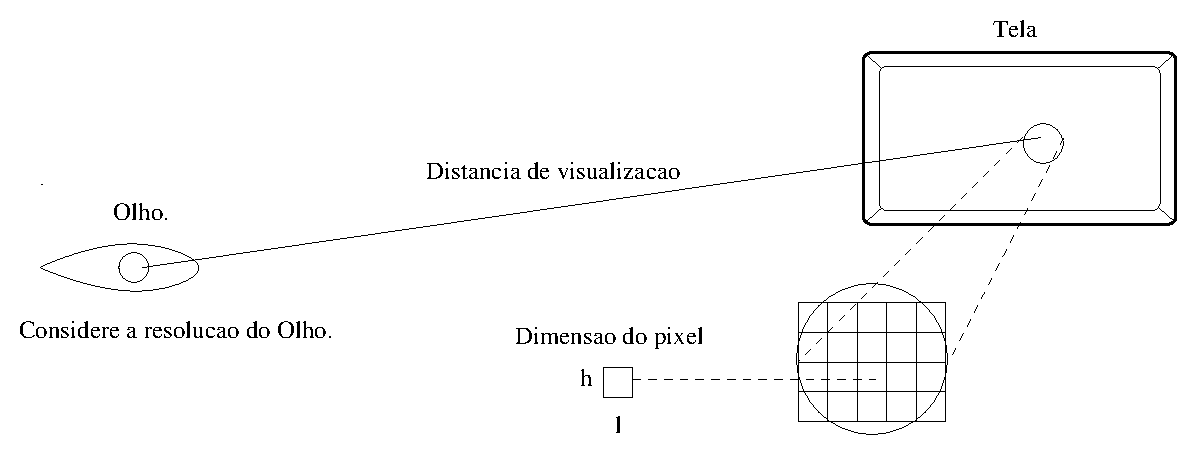
\includegraphics[width=12cm]{./dist_vis.eps}}
\caption{Geometria da visualização de uma imagem em uma tela.}\label{fig:dist_visual}
\end{center}
\end{figure}

\end{enumerate}

%\pagebreak

%\textcolor{red}{Juntar este com o anterior}

%\section{Interpolação de Imagens}


\subsection{Interpolação Usando Médias Ponderadas}

\begin{enumerate}

\item \textbf{Tarefa:} Carregue a imagem \textsf{lena\_256.tif}.  Subamostre-a de 2 em cada direção ({si\-mi\-lar\-men\-te} ao solicitado que vimos na tarefa 5 e mostre a imagem original e a subamostrada simultaneamente.

\item \textbf{Tarefa:} A partir da imagem subamostrada, crie uma imagem com dimensões iguais às da original inserindo uma coluna de zeros à direita de cada coluna e uma linha de zeros abaixo de cada linha. Mostre essa imagem juntamente com as duas acima. 

\item \textbf{Pergunta:} O que você percebe e conclui?

%\item \textbf{Tarefa:} Realize uma subamostragem ainda mais forte retendo apenas um pixel de cada bloco de 8$\times$8 pixeis da imagem.

\item \textbf{Tarefa:} A partir da imagem subamostrada - resultante do item 6.1.1, crie imagens com dimensões iguais às da original inserindo pixeis que valham as \textbf{médias ponderadas} de pixeis vizinhos (usando como referência os pixeis da Figura \ref{fig:pixels_interpol}, na qual $A,~B,~\dots~E $ são os pixeis a criar e $b,~c,~d, \dots m$ são os pixeis presentes na imagem subamostrada). Repare que aqui consideramos dois interpoladores distintos, um usando janelas de 3$\times$3 e outro de 7$\times$7 pixeis. \label{item:interps_def}

\begin{enumerate}
\item Usando uma janela de $3\times 3$ para a interpolação:
\begin{align} A=&\frac{b+c+d+e}{4}, \\ 
 B=&\frac{b+c}{2}, \\
 C=&\frac{d+e}{2}, \\
 D=&\frac{b+d}{2}, \\
 E=&\frac{c+e}{2}.
\end{align}
\item Ou usando uma janela $7\times 7$ para a interpolação:
\begin{align}
A=&\frac{3b+3c+3d+3e+f+g+h+i+j+k+l+m}{20}, \\
B=&\frac{3b+3c+h+i}{8}, \\
C=&\frac{3d+3e+j+k}{8}, \\
D=&\frac{3b+3d+f+l}{8}, \\
E=&\frac{3c+3e+g+m}{8}.
\end{align}

\item\textbf{Obs:} Se um dos pixeis considerados nos modelos acima não existir considere-o zero e faça as correções relevantes para o cálculo da média (isso ocorrerá, por exemplo, nas bordas das imagens).
\end{enumerate}

\begin{figure}[h!]
\begin{center}
{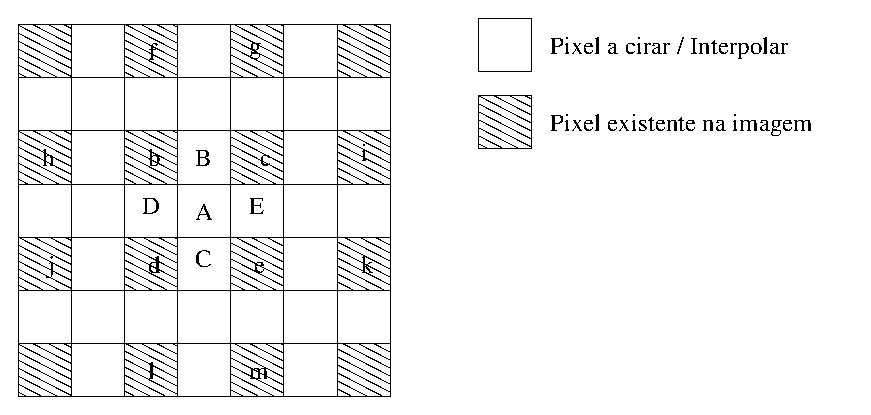
\includegraphics[width=12cm]{./pixels_block.eps}}
\caption{Pixeis considerados nos interpoladores da seção 6.}\label{fig:pixels_interpol}
\end{center}
\end{figure}

\begin{itemize}
\item[\textit{Dica}:] Primeiro gere uma imagem com os pixeis zerados e depois substitua os valores dos pixeis zerados com os calculados usando os interpoladores acima. 

\end{itemize}

\item \textbf{Tarefa:} Mostre as imagens geradas nos itens acima. 
\begin{itemize}
\item[\textit{Dica}:] Lembre-se sempre de mostrá-las em \textsf{truesize} para que uma entrada da matriz que representa a imagem corresponda realmente a um pixel na tela.
\end{itemize}

\item \textbf{Pergunta:} Classifique e discuta a qualidade das imagens geradas através dos procedimentos acima. Discuta a diferença entre os interpoladores empregados.

\end{enumerate}

\subsection{Avaliação de Interpoladores}

\begin{enumerate}

\item \textbf{Tarefa:} Encapsule o processo de interpolação acima em uma função \textrm{Matlab}. Essa função deverá receber uma imagem ou em tons de cinza (uma matriz) ou colorida (isto é três matrizes) e a escolha do tipo de interpolação e retornar as matrizes correspondentes à imagem interpolada. O tipo de variável de saída deverá estar conforme com o de entrada, isto é, se a imagem de entrada for do tipo \textsf{double} a de saída deverá ser \textsf{double} se for do tipo \textsf{uint8} a de saída deverá ser \textsf{uint8}.

\begin{itemize}
\item[\textit{Dica}:] Para lidar com as diferentes possibilidades de chamada e de possíveis saídas (retorno) da função a implementar, veja os comandos \textsf{Matlab}: \textsf{nargin}, \textsf{nargout}, \textsf{nargchk}, \textsf{nargoutchk}, \textsf{varargin} e \textsf{varargout}.

\item[\textit{Dica}:] Para diferenciar o tipo de dados da imagem de entrada use o comando \textsf{isinteger} ou \textsf{isfloat} que permite testar o tipo da variável de entrada.

\end{itemize}

\item \textbf{Tarefa/Pergunta:} Subamostre as imagens \textsf{lena} e \textsf{barbara} até que elas possuam dimensão 64$\times$64. Aplique iteradamente a função acima a essas imagens para obter imagens de dimensões 128$\times$128, 256$\times$256, 512$\times$512, com os interpoladores de janelas quadradas de 3 e 7 pixeis de lado. O que você conclui sobre a qualidade visual das imagens assim geradas?

\end{enumerate}
\end{document}